\section{実装例}

{\system}は、
MacRubyで記述されたMac用日本語IMEである「Gyaim\footnote{
 \textsf{https://github.com/masui/Gyaim}
}」に様々な編集機能を追加して作成した。
本章では{\system}を利用した様々な編集作業の例を示す。
一般にIME はアルファベット以外の文字を入力
するときだけ有効にするのが普通であるが、
ここでは{\system}を常に有効にしておくことにより、
ユーザのあらゆるキー入力を{\system}が取得している。

\subsection{ブロック移動}

テキストの一部を別の場所に移動する操作は
テキストエディタの重要な基本機能のひとつであるが、
エディタによって操作方法が大きく異なっている。
たとえばEmacsでテキストを移動させたい場合は、
移動する領域をキー操作によって指定してから削除/コピーし、
カーソルを移動してからペーストするという手順を利用するが、
ブラウザの編集領域でテキストを移動させたい場合は、
マウスで領域を指定した後で領域をドラッグして別の位置に移動することが多い。
このように、テキスト移動のような基本操作でもエディタごとに操作が異なっているのは不便であるが、
{\system}を利用するとあらゆるエディタで同じ操作でテキストを移動することができる。

図\ref{move1}はMac OSに標準でインストールされている、「テキストエディット」で編集中のテキストである。

\begin{figure}[H]
\centerline{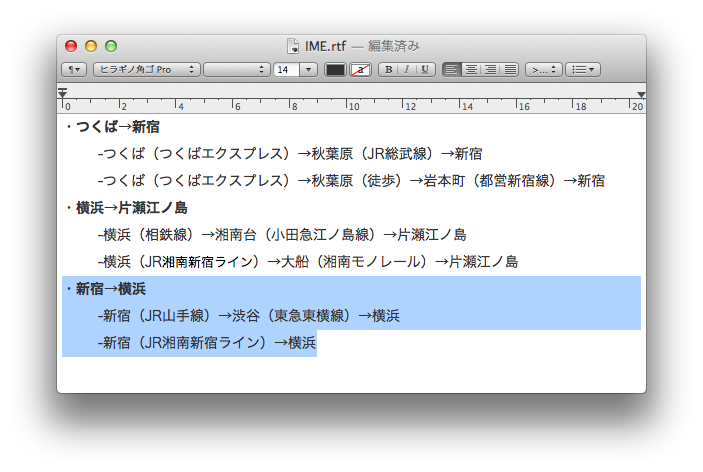
\includegraphics[width=70mm,bb=0 0 703 472]{figures/block2.png}}
\caption{ブロック移動前の状態.}
\label{move1}
\end{figure}

ここでShift+↑キーを押すとテキストは図\ref{move2}のように変化する。

\begin{figure}[H]
\centerline{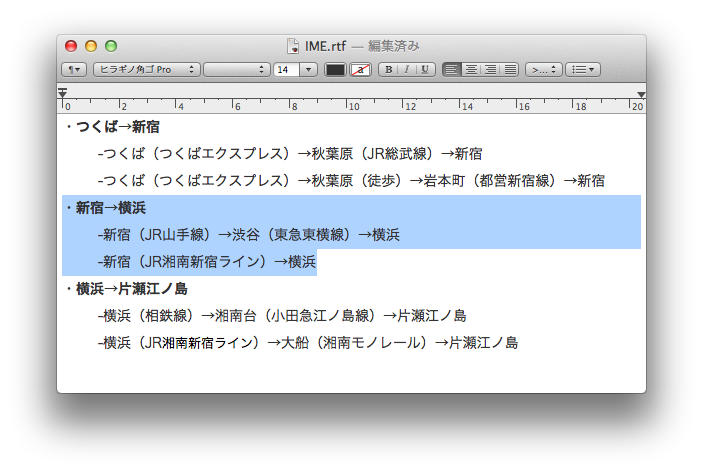
\includegraphics[width=70mm,bb=0 0 703 472]{figures/block3.png}}
\caption{Shift+↑キーを押した後の状態.}
\label{move2}
\end{figure}

図\ref{move3}はブラウザ上でGoogle Docsのテキストを編集しているところである。
ここでShift+↑キーを二度押すと、テキストは図\ref{move4}のように変化する。

\begin{figure}[H]
\centerline{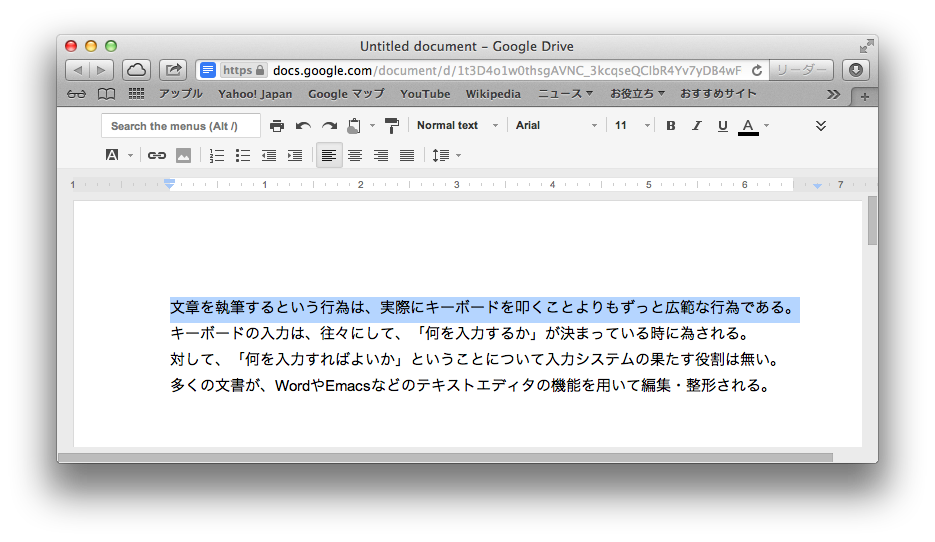
\includegraphics[width=70mm,bb=0 0 935 542]{figures/block4.png}}
\caption{ブロック移動前の状態.}
\label{move3}
\end{figure}

\begin{figure}[H]
\centerline{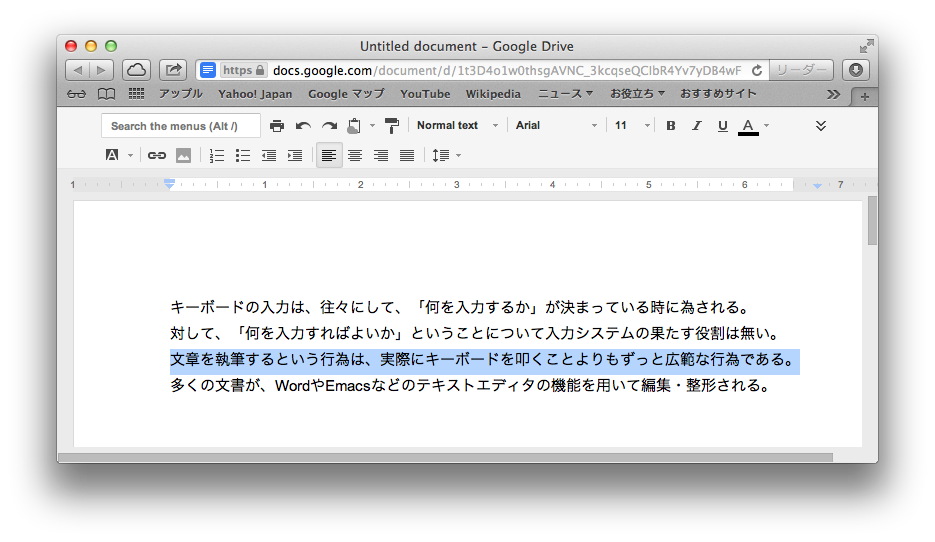
\includegraphics[width=70mm,bb=0 0 935 542]{figures/block5.png}}
\caption{キーを押した後の状態.}
\label{move4}
\end{figure}

このように、あらゆるエディタにおいて同じ操作でブロック移動を行なうことができることがわかる。

\subsection{連続インデント}

前述したブロック移動は、インデントを調整する機能も備えている。
プログラミングを行なっている時だけでなく、
普通のテキストを編集している場合でも
行頭の空白やタブの量を調整するインデント処理は頻繁に行われるが、
自動的にインデントを行うエディタもあれば、
コマンドを打ち込まなければならないものもあり、
そのような調整機能を持っていないエディタも多い。
{\system}を利用すると、あらゆるエディタや入力フィールドでブロック移動と同時にインデントが自動で行われる。

図\ref{indent1}は、Xcode上でPythonプログラムを書いている例である。
Xcodeは、Objective-CやRubyなどの言語で自動インデントの機能を備えているが、Pythonには対応していない。
たとえば、図\ref{indent1}のようなテキストに対して
図\ref{indent2}のように移動させたいブロックを選択し、Shift+↓キーを入力することで、テキストは図\ref{indent3}のように変化する。

\begin{figure}[H]
\centerline{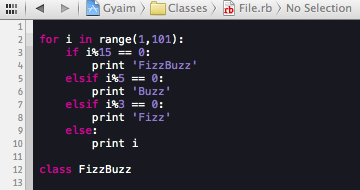
\includegraphics[width=70mm,bb=0 0 360 190]{figures/indent1.png}}
\caption{ブロック移動前の状態}
\label{indent1}
\end{figure}

\begin{figure}[H]
\centerline{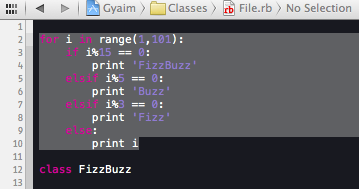
\includegraphics[width=70mm,bb=0 0 360 190]{figures/indent2.png}}
\caption{テキストを選択した状態}
\label{indent2}
\end{figure}

\begin{figure}[H]
\centerline{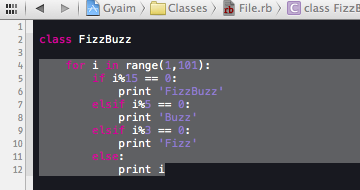
\includegraphics[width=70mm,bb=0 0 360 190]{figures/indent3.png}}
\caption{ブロック移動後の状態}
\label{indent3}
\end{figure}

このように、あらゆるエディタにおいて、ブロック移動を行う際に適切な空白とタブを自動で補完することができる。

\subsection{単語置換}
テキスト編集における単語の検索と置換は、多くのエディタが備えている機能であるが、
その操作方法は異なっている。また、Webブラウザや、
DTPソフトなどでテキストを扱うとき、
検索や置換といった機能は用意されていない。
ブラウザに入力したテキストを、エディタにコピーして編集操作を行うといった作業、あるいはその逆といった作業を{\system}により共通化することが出来る。

以下に{\system}による単語置換の例を示す。図\ref{search1}のように入力語と置換語をテキストエリアに打ち込み、任意に設定したファンクションキーを押すと、
テキストは図\ref{search2}のように置換される。

\begin{figure}[H]
\centerline{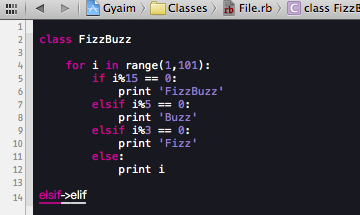
\includegraphics[width=70mm,bb=0 0 360 215]{figures/search_replace1.png}}
\caption{単語置換操作の例}
\label{search1}
\end{figure}

\begin{figure}[H]
\centerline{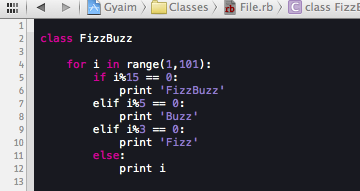
\includegraphics[width=70mm,bb=0 0 360 191]{figures/search_replace2.png}}
\caption{単語置換後の状態}
\label{search2}
\end{figure}

このように、あらゆるエディタ上で検索と置換が可能である。

\subsection{Emacs Lisp}
Emacsにおいてはlisp拡張を導入することでエディタの機能を拡張することが出来るが、これらのスクリプトをIME上に実装することで、他のエディタ上でもこれらの有用な拡張機能を動作させることができる。

以下に{\system}による \cite{DynamicMacro}の例を挙げる。
Dynamic Macroは、入力の繰り返しを自動化するEmacs拡張である。
図\ref{dynamic1}のように、ユーザの入力操作が繰り返しになっているとき、任意に設定したファンクションキーを押すと、テキストは図\ref{dynamic2}のように編集される。

\begin{figure}[H]
\centerline{
\includegraphics[width=80mm,bb=0 0 360 190]{figures/dynamic1.png}}
\caption{Dynamic Macro機能を使用する前のテキスト}
\label{dynamic1}
\end{figure}

\begin{figure}[H]
\centerline{
\includegraphics[width=80mm,bb=0 0 360 190]{figures/dynamic2.png}}
\caption{Dynamic Macro機能を使用した後のテキスト}
\label{dynamic2}
\end{figure}


以下は{\system}のDynamic Macro機能をブラウザのアドレスバー上で実行した例である。
図\ref{dynamic3}のように、ユーザの入力に"abc"が繰り返されているとき、任意に設定したファンクションキーを押すと、テキストは図\ref{dynamic4}のように編集される。

\begin{figure}[H]
\centerline{
\includegraphics[width=70mm,bb=0 0 360 50]{figures/dynamic3.png}}
\caption{Dynamic Macro機能を使用する前のテキスト}
\label{dynamic3}
\end{figure}

\begin{figure}[H]
\centerline{
\includegraphics[width=70mm,bb=0 0 360 50]{figures/dynamic4.png}}
\caption{Dynamic Macro機能を使用した後のテキスト}
\label{dynamic4}
\end{figure}



